%!TEX root = ../report.tex

% 
% Architecture
% 

\section{Architecture}

%introduction
This section proposes a solution to solve the need of a refactoring tool designed for inexperienced users.
%A refactoring tool that would suit an inexperienced programmer who is learning how to program is needed.
Because it is targeted for inexperienced users it is important to have an environment that is not complex like Eclipse and to be for a programing language that is used in introductory courses, such as Python and Racket.
Racket is a dynamic language that is known for being used as in introductory programming courses in schools around the world. 
Racket has an IDE, DrRacket, that is a pedagogic environment \cite{drscheme_pegadogy} and it also supports development and extension of other programming languages \cite{tobin2011languages}. 
Recently  an implementation of Python for Racket was added \cite{ramos2014implementation}. 
This addition makes it possible to have Python programs in DrRacket and with that the pedagogical environment gains another language that is used in introductory courses around the world. Because of that DrRacket environment was chosen. 
Racket programming language was chosen because it is easier to create refactoring operations for Racket in the DrRacket environment.
This tool will motivate the inexperienced programmers to start using tool assisted refactoring operations and DrRacket seams to be the ideal candidate to have that refactoring tool.


%use cases: To validate the architecture.
\subsection{Refactoring Operations}
%Das operacoes para a refactoring tool vamos falar particularmente destas, ou por exemplo destas.
The refactoring tool consists in a set of refactoring operations.
This section describes some of the refactoring operations desired and their use.
%introduce the validate cases xD

% rename improved
\subsubsection{Rename}
\label{ssub:Rename}
%this is a refactoring for racket
is the most used refactoring operation and it is indispensable in any refactoring tool.
The DrRacket environment already has a rename operation, however the rename has a bug when renaming imported functions.
This bug, as it can be seen in Figure~\ref{fig:RacketBug} happens when the user renames an imported function, with the original rename operation of DrRacket, it renames all the imported functions from the same file and it also renames the name of the imported file.
This is an incorrect refactoring because it makes the program syntactically incorrect. It should only rename the function with the selected name, not every function from that file.
This situation may occur when using functions from other file, whether there is a name conflict or because it is better for the readability to rename that function name.
%After that, the user can call the methods exported like they were defined in the file.
%However those methods could have name collision or change it for a more adequate name. To do that the user would do a rename.
\begin{figure}[htbp]
	\centering
	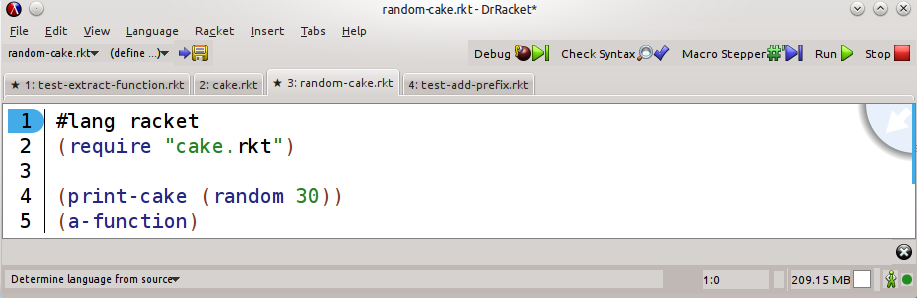
\includegraphics[width=0.9\textwidth]{img/renameV2-1.png}
	\caption{Before the Rename}
	\label{fig:renameBefore}
\end{figure}

\begin{figure}[htbp]
	\centering
	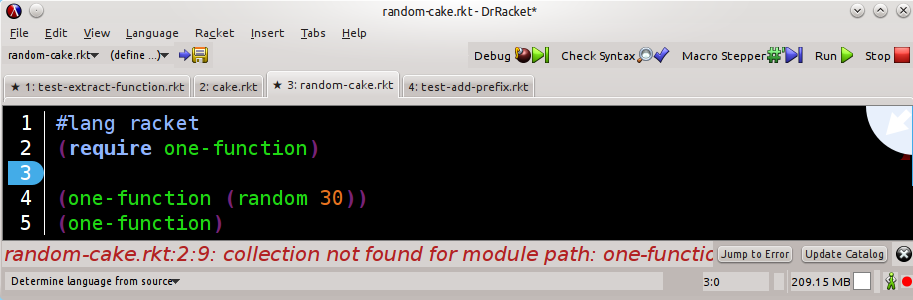
\includegraphics[width=0.9\textwidth]{img/rename-error.png}
	\caption{Rename error on DrRacket}
	\label{fig:RacketBug}
\end{figure}

% extract-function
\subsubsection{Extract-function}

is a simple and useful refactoring, as shown previously in Section~\ref{sec:Introduction}, it is one of the most used refactoring operations.

Extract-function is an important refactoring for inexperienced users since those users tend to create a big function that does all the work.

By having a way to restructure the code, inexperienced programmers will be able to create programs with better structures.




\subsubsection{Move expression}

is also one of the most used refactoring operations.
This operation allows the user to move safely the expressions, by correcting all references, to the new location. 



% add-prefix
\subsubsection{Add-prefix}
%this is a refactoring for racket only!
is a particular refactoring operation for Racket.
%When using two libraries that have functions with the same name there is a naming conflict.
%This happens when a programmer is using some functions from a library and then realizes that needs another function.
%The new function has the same name of one of the used functions and that creates a conflict error.
%The solution is to add a prefix for one of the imported libraries.
When several functions are imported from several different libraries the code starts to become difficult to understand.
With so many functions from different libraries it is hard to remember where a specific function came from.
To solve this problem, Racket has a prefix that can be added to the imported functions.
This prefix helps improving the readability of the code and, therefore, the code's quality.
However, doing that manually is a tiresome task because the user has to remember and change one by one all function invocations.

The Add Prefix refactoring does all that for the user.
This is also useful when the name of the functions are similar, adding a prefix makes it easier to distinguish between libraries.





\subsection{Proposed Architecture}
%s-exp and def-uses-relationships

%An image will be awesome here
Figure~\ref{fig:architecture} presents the proposed architecture of the tool. 
The refactoring tool uses, mainly, two important informations gathered by the compiler, the def-use-relations and the AST.
A def-use-relation consists in a definition of a variable and all the uses that reach the variable without any intervening definitions.
The information gathered in the AST and in the def-use-relations with some preconditions is enough to ensure the correctness of the refactoring operations.
The refactoring tool uses the information generated by the compiler and some conditions to ensure that the refactoring is correct. After that it changes the program creating another version.
The AST in the Racket programing language composed by a list of s-expressions, which are basically a nested list of basic data, and have the syntax information about the program and other useful information such as in which line and column a term is declared.
DrRacket provides the def-use-relations which is an important help to do the refactoring operations. 
The def-use-relations are visually represented as arrows in DrRacket.

\begin{figure}[htbp]
	\centering
	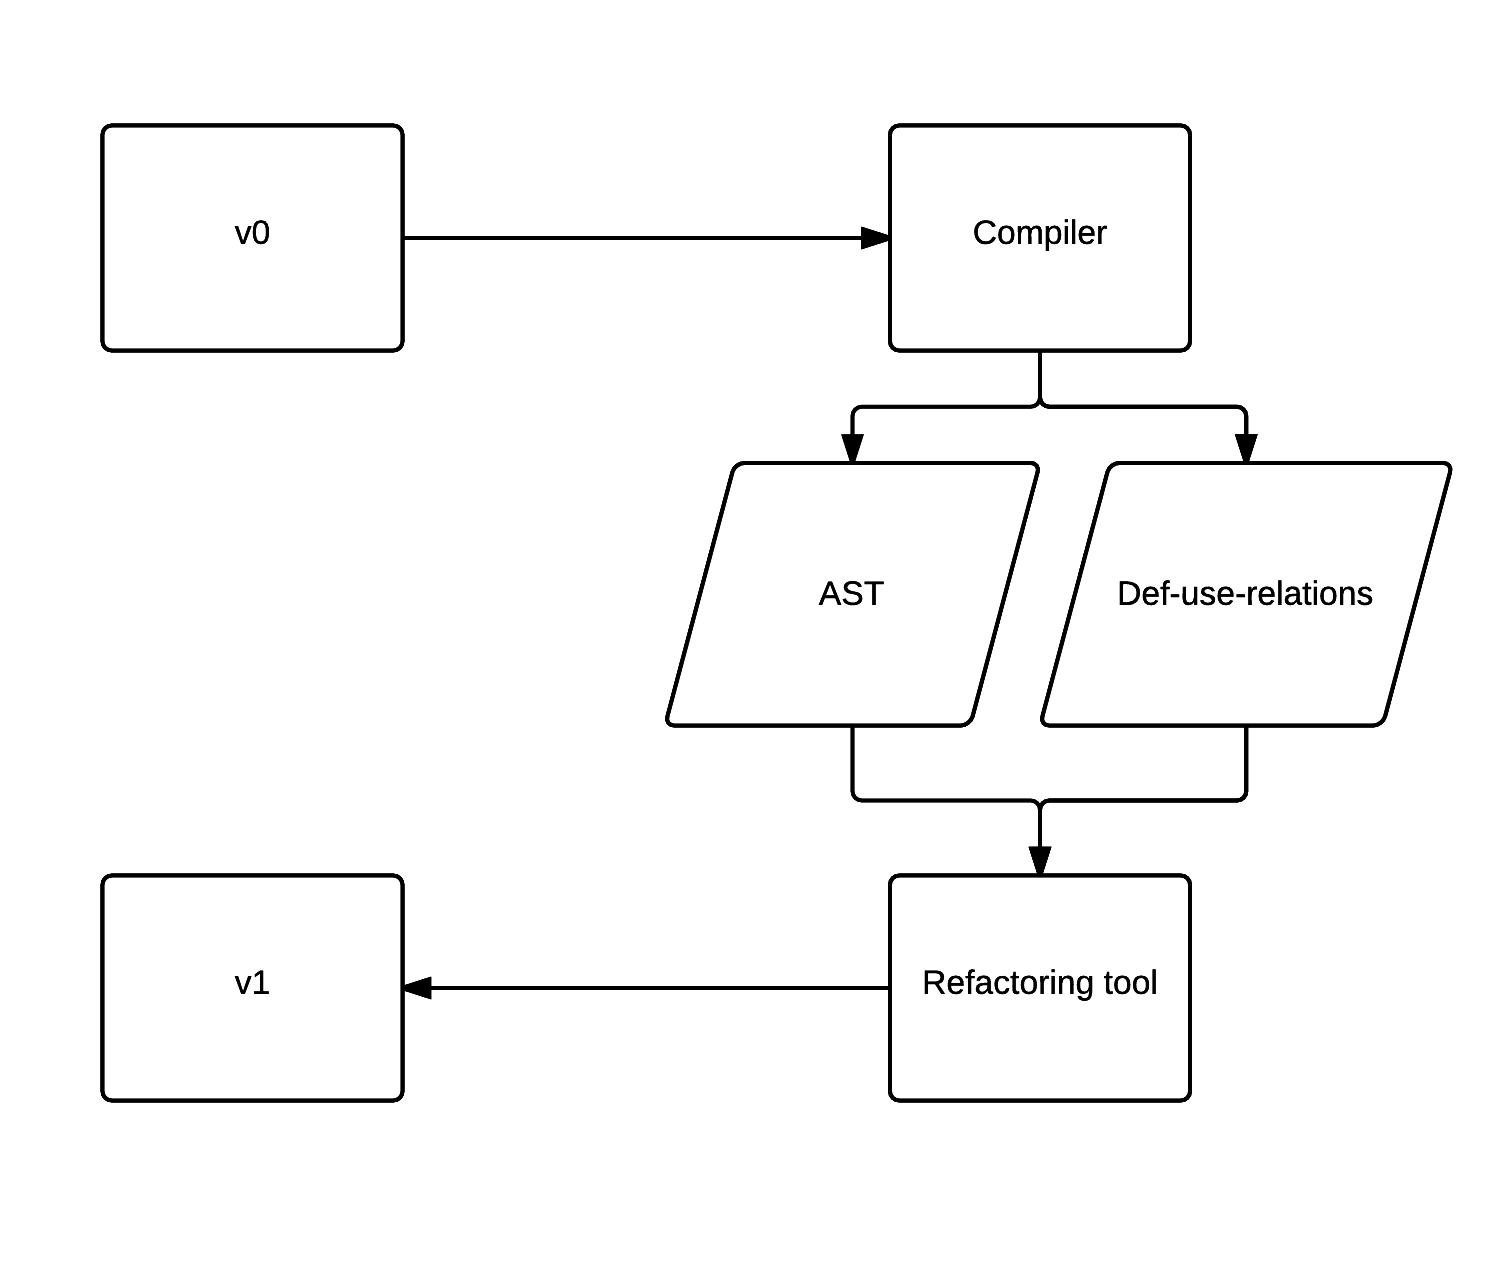
\includegraphics[width=0.9\textwidth]{img/arquitectura.png}
	\caption{The arrows determines the information flow; v0 is the initial program; The compiler produces two databases the AST and the Def-use-relations; The Refactoring Tool use the AST and the Def-use-relations produced by the compiler to generate v1, which is the refactored program}
	\label{fig:architecture}
\end{figure}


\subsection{Validation}
%In order to evaluate it was implemented a prototype in DrRacket.
In order to validate this architecture some refactoring operations were implemented. 
This allow us to validate the architecture and have more trust in this architecture.
Only the refactoring operations that use exclusively the def-use-relations were validated.

\subsubsection{Extract-function}
The user selects the expressions that wants to extract and chooses a name for the new function as seen in {\bf Figure~\ref{fig:extractBefore}}.
Then the user pastes the result of the extraction where he thinks it's the best place for the function. 
The final result can be seen in {\bf Figure~\ref{fig:extractAfter}}.
The extract function refactoring could automatically paste the extracted function, however this way the user can choose the function's location.
\begin{figure}[htbp]
	\centering
	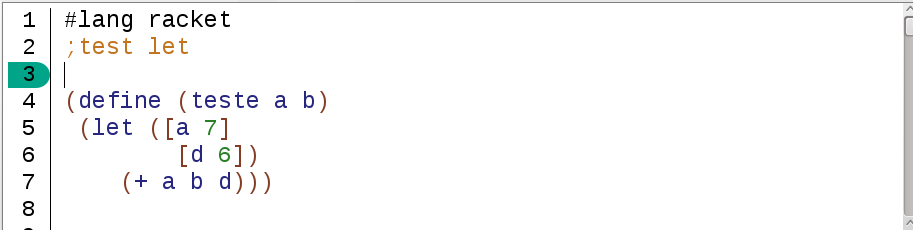
\includegraphics[width=0.9\textwidth]{img/extractV3.png}
	\caption{Before the Extract function}
	\label{fig:extractBefore}
\end{figure}

\begin{figure}[htbp]
	\centering
	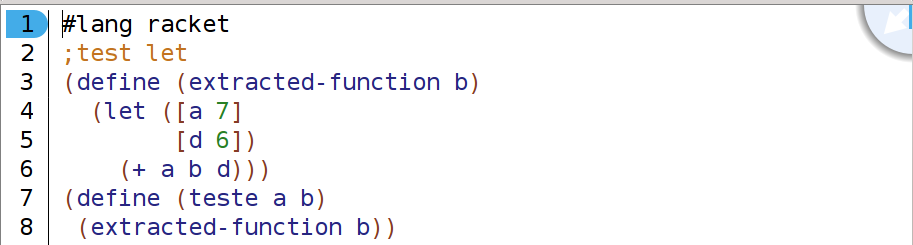
\includegraphics[width=0.9\textwidth]{img/extractV2-2.png}
	\caption{After the Extract function}
	\label{fig:extractAfter}
\end{figure}

\subsubsection{Imported renames}
As explained in ~\ref{ssub:Rename} the only refactoring operation supported by DrRacket, the Rename, has bugs when it has to rename imported functions.
To do the rename, the user selects the function that wants to be renamed, as seen in {\bf Figure~\ref{fig:renameBefore}} and in this case the user chose ``print-cake''.
Afterwards the user chooses the name that wants go give and finally it renames all the functions. 
The end result is shown in {\bf Figure~\ref{fig:renameAfter}}.

\begin{figure}[htbp]
	\centering
	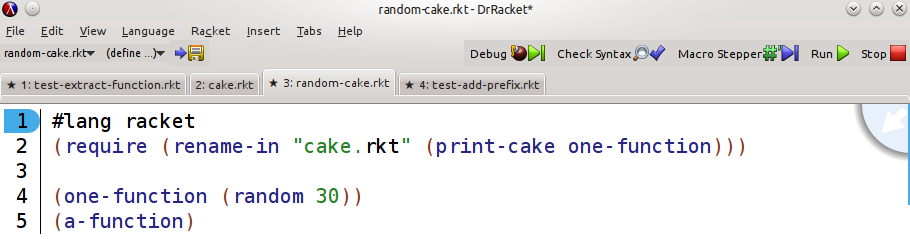
\includegraphics[width=0.9\textwidth]{img/renameV2-2.png}
	\caption{After the Rename}
	\label{fig:renameAfter}
\end{figure}

\subsubsection{Add-prefix}

This is a particular refactoring operation for Racket. Adding a prefix is normally used when there are naming conflicts with two different libraries. The user goes to the library name, and adds a prefix.
In {\bf Figure~\ref{fig:addPrefixBefore}} the arrows show which functions belong to the ``pict3d'' library.
Then the user selects a name for the prefix that name will be added, and then the final result is shown in {\bf Figure~\ref{fig:addPrefixAfter}}.

\begin{figure}[hb!]
	\centering
	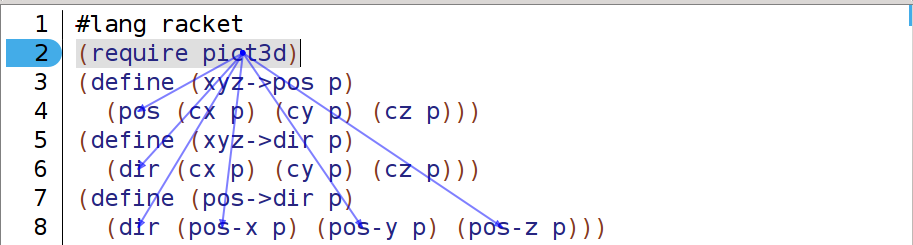
\includegraphics[width=0.9\textwidth]{img/add-prefixV2-1.png}
	\caption{Before adding the prefix}
	\label{fig:addPrefixBefore}
\end{figure}

%\begin{figure}[htbp]
%	\centering
%	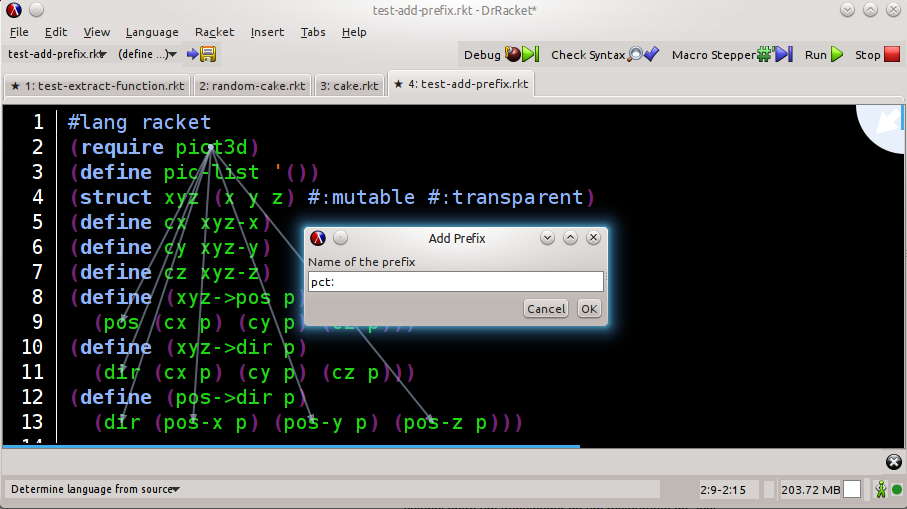
\includegraphics[width=0.8\textwidth]{img/add-prefixV2-2.png}
%	\caption{Choosing the prefix}
%	\label{fig:addPrefixDuring}
%\end{figure}

\begin{figure}[hb!]
	\centering
	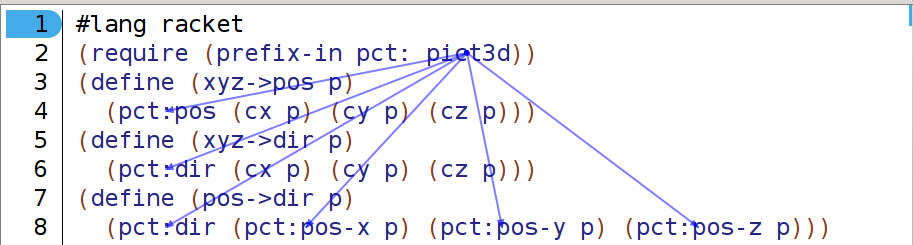
\includegraphics[width=0.9\textwidth]{img/add-prefixV2-3.png}
	\caption{After the Add-prefix refactoring}
	\label{fig:addPrefixAfter}
\end{figure}